\documentclass{article}
\usepackage{tikz}
\usetikzlibrary{automata,positioning,arrows}

% \tikzset{every edge/.append style={
%   auto,
% }}

\begin{document}

\section{Example 1: $(a^\sharp\{a,b\})^\sharp$} 
%
%% Machine generated by https://finsm.io
%% 2025-3-21-5:56:39
%% include in preamble:
%% \usepackage{tikz}
%% \usetikzlibrary{automata,positioning,arrows}
%% (a#{a,b})#
\begin{center}
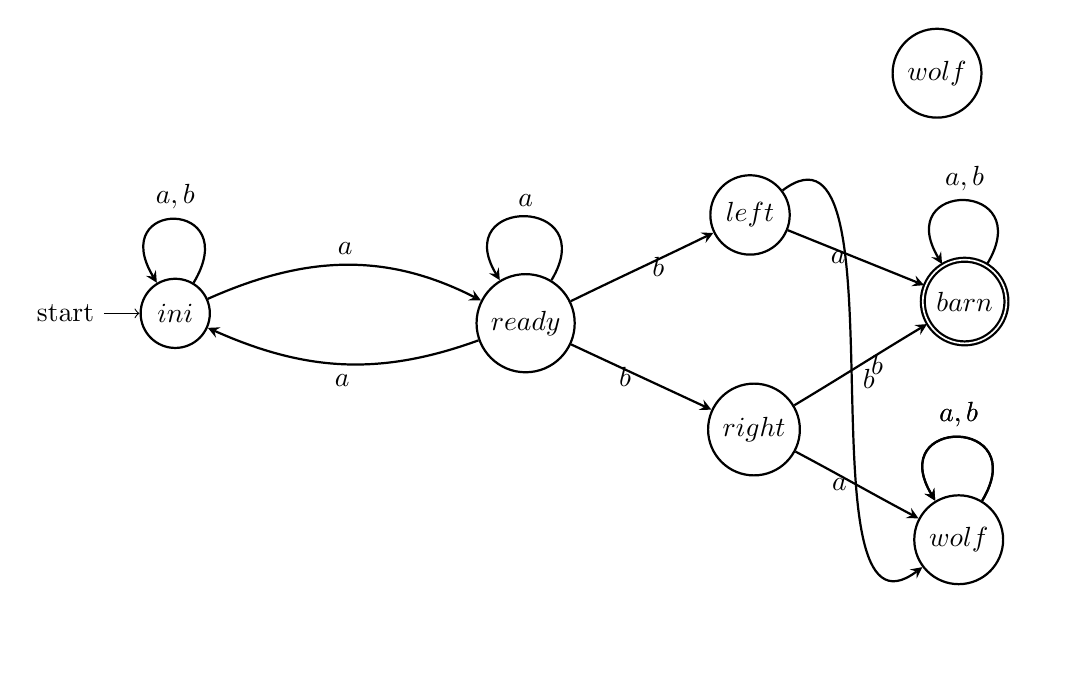
\begin{tikzpicture}[]
    \node[initial,thick,state] at (-3.175,4.95) (1fa0116c) {$ini$};
    \node[thick,state] at (1.275,4.825) (4c126865) {$ready$};
    \node[thick,accepting,state] at (6.85,5.1) (b8befb7d) {$barn$};
    \node[thick,state] at (4.125,6.2) (316b0ce4) {$left$};
    \node[thick,state] at (4.175,3.475) (6e65ff45) {$right$};
    \node[thick,state] at (6.5,8) (8a7c360d) {$wolf$};
    \node[thick,state] at (6.775,2.075) (8a7c360d) {$wolf$};
    \path[->, thick, >=stealth]
    (1fa0116c) edge [loop,min distance = 1.25cm,above,in = 121, out = 59] node {$a,b$} (1fa0116c)
    (1fa0116c) edge [above,in = 153, out = 24] node {$a$} (4c126865)
    (4c126865) edge [loop,min distance = 1.25cm,above,in = 121, out = 59] node {$a$} (4c126865)
    (4c126865) edge [below,in = -24, out = -160] node {$a$} (1fa0116c)
    (4c126865) edge [right,in = -154, out = 26] node {$b$} (316b0ce4)
    (4c126865) edge [left,in = 155, out = -25] node {$b$} (6e65ff45)
    (b8befb7d) edge [loop,min distance = 1.25cm,above,in = 121, out = 59] node {$a,b$} (b8befb7d)
    (316b0ce4) edge [left,in = 158, out = -22] node {$a$} (b8befb7d)
    (316b0ce4) edge [right,in = -143, out = 37] node {$b$} (8a7c360d)
    (6e65ff45) edge [right,in = -149, out = 31] node {$b$} (b8befb7d)
    (6e65ff45) edge [left,in = 152, out = -28] node {$a$} (8a7c360d)
    (8a7c360d) edge [loop,min distance = 1.25cm,above,in = 121, out = 59] node {$a,b$} (8a7c360d)
    (8a7c360d) edge [loop,min distance = 1.25cm,above,in = 121, out = 59] node {$a,b$} (8a7c360d)
    ;
\end{tikzpicture}
\end{center} 



\section{Example 2: capacity-1 bottlenecks}

\subsection{The most basic version}
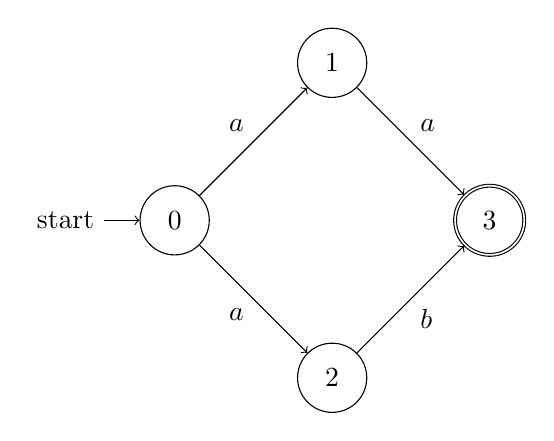
\begin{tikzpicture}[
    every edge/.style={draw,auto}
]
	\node[state, initial] at (0,0) (A) {$0$};

	\node[state] at (2,2) (B) {$1$};
	
	\node[state] at (2,-2) (C) {$2$};
	
	\node[state,accepting] at (4,0) (D) {$3$};
    
	\path[->]
	(A) edge [] node {$a$} (B)
	(A) edge [swap] node {$a$} (C)
	(B) edge [] node {$a$} (D)
	(C) edge [swap] node {$b$} (D)
    ;
\end{tikzpicture}

 

\subsection{The same basic version but complete}
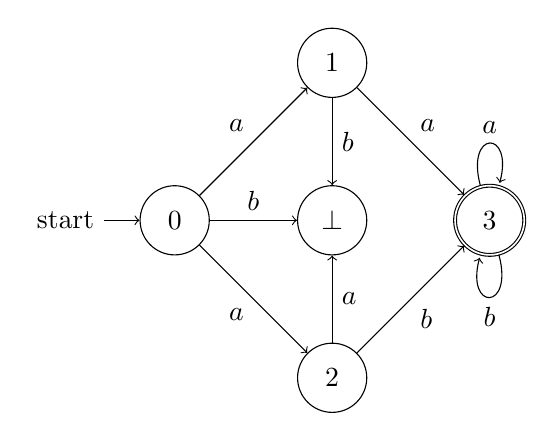
\begin{tikzpicture}[
    every edge/.style={draw,auto}
]
	\node[state, initial] at (0,0) (A)  {$0$};
	\node[state] at (2,2) (B)  {$1$};
	\node[state] at (2,-2) (C) {$2$};
	\node[state,accepting] at (4,0) (D)  {$3$};
	\node[state] at (2,0) (BOT) {$\bot$};
    \path[->]
	(A) edge node[] {$a$} (B)
	(A) edge node[swap] {$a$} (C)
	(A) edge node[] {$b$} (BOT)
	(B) edge node[] {$a$} (D)
	(B) edge node[] {$b$} (BOT)
	(C) edge node[swap] {$b$} (D)
	(C) edge node[swap] {$a$} (BOT)

	(D) edge[loop above] node[swap] {$a$} (D)
	(D) edge[loop below] node[swap] {$b$} (D)
    ;
\end{tikzpicture}
 

\subsection{The same basic version, generated in finsm.io}
%% Machine generated by https://finsm.io
%% 2025-3-23-4:04:031
%% include in preamble:
%% \usepackage{tikz}
%% \usetikzlibrary{automata,positioning,arrows}
\begin{center}
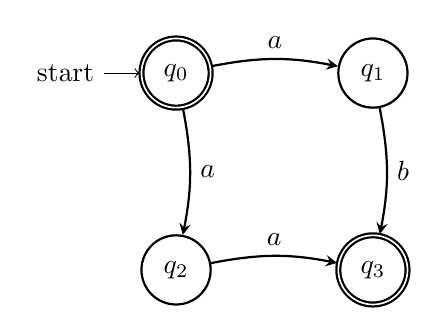
\begin{tikzpicture}[]
    \node[initial,thick,accepting,state] at (-1.25,1.25) (534d1af6) {$q_0$};
    \node[thick,state] at (1.25,1.25) (8f1120a5) {$q_1$};
    \node[thick,state] at (-1.25,-1.25) (0776f76f) {$q_2$};
    \node[thick,accepting,state] at (1.25,-1.25) (8b23c0f0) {$q_3$};
    \path[->, thick, >=stealth]
    (534d1af6) edge [above,in = 169, out = 11] node {$a$} (8f1120a5)
    (534d1af6) edge [right,in = 79, out = -79] node {$a$} (0776f76f)
    (8f1120a5) edge [right,in = 79, out = -79] node {$b$} (8b23c0f0)
    (0776f76f) edge [above,in = 169, out = 11] node {$a$} (8b23c0f0)
    ;
\end{tikzpicture}
\end{center}
 

\subsection{The version as appears in the paper, with alphabet $\{a,b,c,d,e\}$.}
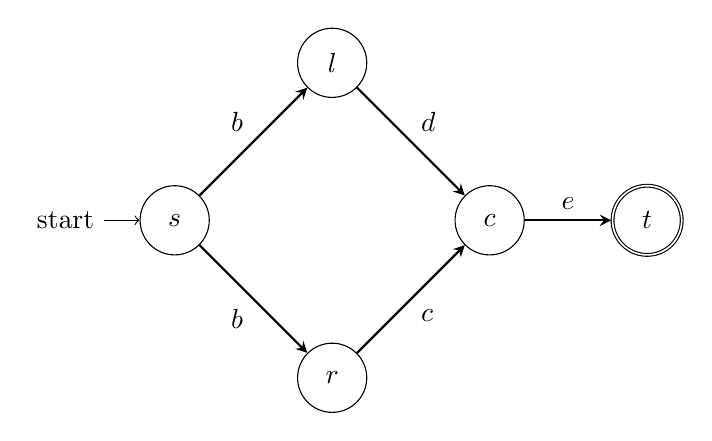
\begin{tikzpicture}[
    every edge/.style={draw,auto}
]
	\node[state, initial] (A) at (0,0) {$s$};
	\node[state] at (2,2) (B)  {$l$};
	\node[state] at (2,-2) (C) {$r$};
	\node[state] at (4,0) (D)  {$c$};
	\node[state,accepting] at (6,0) (E) {$t$};
    \path[->, thick, >=stealth]
	(A) edge node[] {$b$} (B)
	(A) edge node[swap] {$b$} (C)
	(B) edge node[] {$d$} (D)
	(C) edge node[swap] {$c$} (D)
	(D) edge node[] {$e$} (E)
    ;
\end{tikzpicture}
 

\subsection{The paper version but complete.}
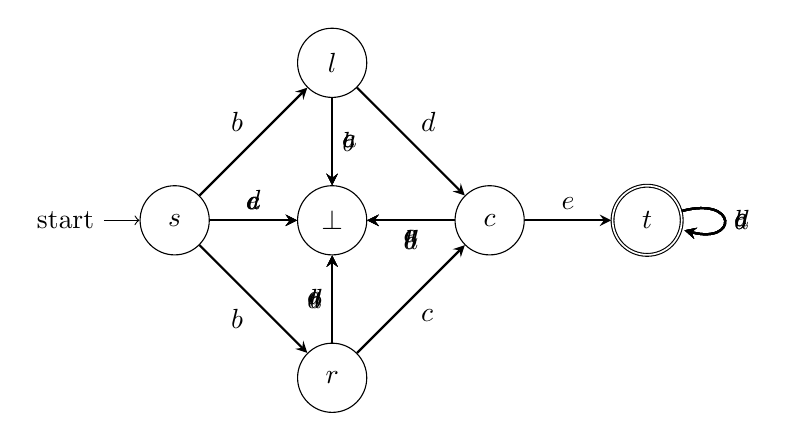
\begin{tikzpicture}[
    every edge/.style={draw,auto}
]
	\node[state, initial] at (0,0) (A) {$s$};
	\node[state] at (2,2) (B)  {$l$};
	\node[state] at (2,-2) (C) {$r$};
	\node[state] at (4,0) (D)  {$c$};
	\node[state,accepting] at (6,0) (E) {$t$};
	\node[state] at (2,0) (BOT) {$\bot$};

    \path[->, thick, >=stealth]
	(A) edge node[] {$b$} (B)
	(A) edge node[swap] {$b$} (C)
	(B) edge node[] {$d$} (D)
	(C) edge node[swap] {$c$} (D)
	(D) edge node[] {$e$} (E)
	(A) edge node[] {$a$} (BOT)
	(A) edge node[] {$c$} (BOT)
	(A) edge node[] {$d$} (BOT)
	(A) edge node[] {$e$} (BOT)
	(B) edge node[] {$a$} (BOT)
	(B) edge node[] {$b$} (BOT)
	(B) edge node[] {$c$} (BOT)
	(B) edge node[] {$e$} (BOT)
	(C) edge node[] {$a$} (BOT)
	(C) edge node[] {$b$} (BOT)
	(C) edge node[] {$d$} (BOT)
	(C) edge node[] {$e$} (BOT)
	(D) edge node[] {$a$} (BOT)
	(D) edge node[] {$b$} (BOT)
	(D) edge node[] {$d$} (BOT)
	(D) edge node[] {$e$} (BOT)
	(E) edge[loop right] node[swap] {$a$} (E)
	(E) edge[loop right] node[swap] {$b$} (E)
	(E) edge[loop right] node[swap] {$c$} (E)
	(E) edge[loop right] node[swap] {$d$} (E)
	(E) edge[loop right] node[swap] {$e$} (E)
    ;
\end{tikzpicture}
 
\end{document}
